\documentclass[a4paper, twoside]{article} %classe du document
%a4paper format A4 de la page

%extensions
\usepackage{eso-pic} % For \AddToShipoutPicture used for cover backgrounds
\usepackage[utf8]{inputenc} %encodage d'entrée
\usepackage[french]{babel}
\usepackage{ae,lmodern}
\usepackage[T1]{fontenc} %encodage de sortie
\usepackage{amsthm,amsmath,amsfonts,amssymb,mathtools} %extension pour les maths
\usepackage{graphicx} %extension pour les images
\usepackage{xcolor} %extension pour les couleurs
\usepackage{hyperref}
\usepackage[left=1.3cm, right=1.3cm, top=1.3cm, bottom=1.3cm]{geometry}%marges
\usepackage{colortbl}
\graphicspath{ {./img/} }
\usepackage{listings} % Permet d'ajouter du code
\usepackage{float} % place correctement les images

\usepackage{lipsum} % pour tester avec du texte factice

\definecolor{codegreen}{rgb}{0,0.6,0}
\definecolor{codegray}{rgb}{0.5,0.5,0.5}
\definecolor{codepurple}{rgb}{0.58,0,0.82}
\definecolor{backcolour}{rgb}{0.95,0.95,0.92}

\lstdefinestyle{mystyle}{
    backgroundcolor=\color{backcolour},   
    commentstyle=\color{codegreen},
    keywordstyle=\color{magenta},
    numberstyle=\tiny\color{codegray},
    stringstyle=\color{codepurple},
    basicstyle=\ttfamily\footnotesize,
    breakatwhitespace=false,         
    breaklines=true,                 
    captionpos=b,                    
    keepspaces=true,                 
    numbers=left,                    
    numbersep=5pt,                  
    showspaces=false,                
    showstringspaces=false,
    showtabs=false,                  
    tabsize=2
}

\lstset{
        literate=
        {à}{{\`a}}1
        {é}{{\'e}}1
        {è}{{\`e}}1
        {ù}{{\`u}}1,
        style=mystyle
     }

\begin{document}

\AddToShipoutPicture*{
    \put(0,0){
\includegraphics[width=\paperwidth,height=\paperheight,keepaspectratio]{img/back-background.pdf}}
}

\begin{figure}[t]
	\begin{minipage}[b]{0.2\linewidth}
		\raggedright 
\includegraphics[scale=0.5]{enib.jpg}
	\end{minipage}\hfill
	\begin{minipage}[b]{0.4\linewidth}	
		\raggedleft 
\includegraphics[scale=0.5]{logo.jpg}
	\end{minipage}
\end{figure}

\begin{titlepage}
\begin{center}
ENIB semestre SXX : \\
XXX(nom du bloc) - XXX (matière)\\
\vspace{2cm}
\huge{\textsl{NOM PROJET}\textbf{ : \\
Decription du projet}}\\
\end{center}
\begin{center}
\rule{\linewidth}{1pt}
\end{center}

\begin{minipage}[t]{0.47\textwidth}
	{\large George Lumière}
\end{minipage}\hfill
\begin{minipage}[t]{0.47\textwidth}\raggedleft
	{\large SXX-X}
\end{minipage}

\vspace{2.5cm}

\begin{figure}[H]
	\centering 
\includegraphics[width=0.8\textwidth]{guardpage.jpg}
\end{figure}

\vspace{0.3cm}

\centering{Version X.0 : XX XXX 202X}
\end{titlepage}

%affichage du sommaire
\tableofcontents
\listoffigures

\newpage

\section{\lipsum[1][1]}
\lipsum[3-5]

\begin{figure}[H]
\begin{center}
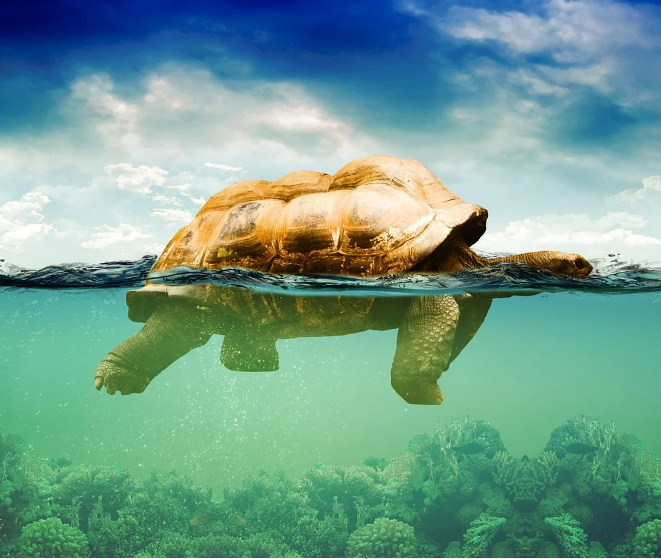
\includegraphics[height=7cm]{img/fig.jpg}\\
\caption{\lipsum[1][4]}
\end{center}
\end{figure}

\lipsum[5-6]\\

\lstinputlisting[language=Python]{py/example.py}

\end{document}